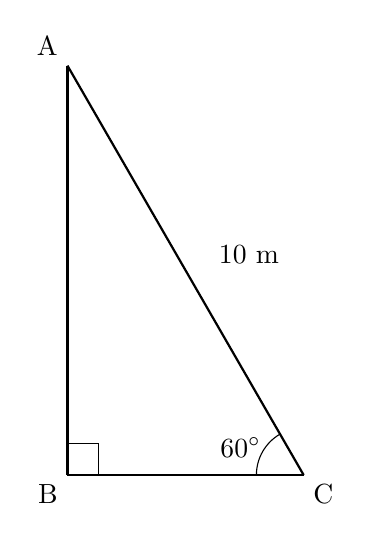
\begin{tikzpicture}

    % Define the coordinates for the right triangle
    \coordinate (B) at (0, 0);       % Bottom left vertex (right angle)
    \coordinate (C) at (3, 0);       % Bottom right vertex
    \coordinate (A) at (0, 5.2);     % Top vertex
    
    % Draw the triangle sides
    \draw[thick] (A) -- (B);         % Side AB (vertical)
    \draw[thick] (B) -- (C);         % Side BC (horizontal)
    \draw[thick] (A) -- (C);         % Side AC (hypotenuse)
    
    % Draw the right angle symbol at B
    \draw (0, 0.4) -- (0.4, 0.4) -- (0.4, 0);
    
    % Draw the arc for 60 degree angle at C
    \draw (2.4, 0) arc (180:120:0.6);
    
    % Label point A
    \node[above left] at (A) {A};
    
    % Label point B
    \node[below left] at (B) {B};
    
    % Label point C
    \node[below right] at (C) {C};
    
    % Label the 60 degree angle at C
    \node at (2.2, 0.35) {$60^{\circ}$};
    
    % Label the hypotenuse with 10.
    \node[right] at (1.8, 2.8) {10 \text{m}};
    
    \end{tikzpicture}